\documentclass[journal, compsoc]{IEEEtran}
\documentclass{article}

\usepackage[utf8]{inputenc}
\usepackage{longtable}
\usepackage{graphicx}
\usepackage{algorithm}
\usepackage{graphicx}
\usepackage{algorithm}
\usepackage{algpseudocode}
\usepackage{amsmath}
\usepackage{amsfonts}
\usepackage{hyperref}
\usepackage{mathtools}
\usepackage[euler-digits,euler-hat-accent]{eulervm}

\bibliographystyle{IEEEtran}

\DeclareMathOperator*{\argmin}{arg\,min}
\newcommand\Mycomb[2][^n]{\prescript{#1\mkern-0.5mu}{}C_{#2}}

\title{Artificial Intelligence Report on Solutions to Laboratory Problems}

\author{Siddhartha~Tiwari, Siddharth~Mani~Tiwari, Saurabh~Kumar, Pushkar~Tiwari}

%\author{
%\IEEEauthorblockN{Siddhartha Tiwari}\IEEEauthorblockA{201851127}
%\and
%\IEEEauthorblockN{Siddharth Mani Tiwari}\IEEEauthorblockA{201851126}
%\and
%\IEEEauthorblockN{Saurabh Kumar}\IEEEauthorblockA{201851113}
%\and
%\IEEEauthorblockN{Pushkar Tiwari}\IEEEauthorblockA{201851095}
%}

\begin{document}
\IEEEtitleabstractindextext{%
\begin{abstract}
This report is the part two of discussions on laboratory problems assigned to us by Dr. Pratik Shah. The problems discussed are from various fields including Hidden Markov Models, Markov Random Fields, Hopfield Networks, Unsupervised Learning, N-Arm Bandit e.t.c. For each problem, the most efficient solution is arrived upon gradually, using different techniques taught in the class.
\end{abstract}
}
\maketitle

\section{Hidden Markov Models and Expectation Maximization}
\subsection{Finding structures in the English language using Hidden Markov Models}
\subsubsection{Introduction}
In this problem, we are trying to use the Hidden Markov Models to predict the structure of English Languague. Initially we are not assuming anything about the structure and doing the experiment based
on a large collection of words ($50,000$ to be exact) extracted from the book War and Peace by Leo Tolstoy. There are two hidden states (details in the next section) and the observation sequence
(obtained by words extracted) contains all the $26$ letters of the English language plus the space character. And these characters are mapped to indices from 0 to 26 where 0 represents the letter 'a' and
26 is the space.
\subsubsection{Forward \& Backward algorithms}
Let $O$ represents the observation sequence, $\lambda = (\pi, A, B)$ represents the model, where $A$ is the matrix containing the transition probabilities, $B$ is the matrix containing the emission
probabilities and $\pi$ is the initial state probabilities.

Now in order to infer anything about the hidden states in Hidden Markov Models, we first have to find out how to find the probabilities ${\gamma_t(i) = P(x_t = q_i | O, \lambda)}$ and ${\gamma_t(i, j) = P(x_t = q_i, x_{t + 1} = q_j | O, \lambda)}$.
The first term $\gamma_t(i)$ is the probability of being in the $i^{th}$ hidden state at time $t$, given the model and the observation sequence. The second term $\gamma_t(i, j)$ represents the probability of being in the $i^{th}$ state at time $t$ and then
transiting to the $j^{th}$ state at time $t + 1$. These probabilities enable us to compute the matrices $A$, $B$ and $\pi$ and thus to reestime the model. Thus we can use expectation maximization to estimate the models if these two probabilities are available.
But calculating the probabilities is not straight forward and the naive algorithm to calculate the given probabilities will take a great amount of time. So, to calculate these two probabilities we will first calculate the alpha-pass (or the Forward algorithm) and the beta-pass (the Backward algorithm):
\begin{equation}
\begin{aligned}
    \alpha_t(i) &= P(O_0, O_1, O_2, \ldots, O_t, x_t = q_i | \lambda)\\
    \beta_t(i) &= P(O_{t + 1}, O_{t + 2}, O_{t + 3}, \ldots, O_{T - 1} | x_{t} = q_i, \lambda)
\end{aligned}
\end{equation}

The reason to calculate the alpha and beta pass is that these probabilities can be easily expressed recursively and thus can greatly reduce the time required to calculate these probabilities. Also, the probabilities $\gamma_t(i)$ and $\gamma_t(i, j)$ can be
expressed in terms of these alpha and beta pass along with the probability $P(O | \lambda)$ is given in the equation \ref{eqn:express}.
\begin{equation}
\label{eqn:express}
\begin{aligned}
P(O | \lambda) &= \sum_{i = 0}^{N}\alpha_{T - 1}(i)\\
\gamma_t(i) &= \frac{\alpha_t(i)\cdot \beta_t(i)}{P(O | \lambda)}\\
\end{aligned}
\end{equation}
\begin{equation}
\begin{aligned}
    \gamma_t(i, j) = \frac{\alpha_t(i)\cdot a_{ij}\cdot b_j(O_{t + 1}) \cdot \beta_{t + 1}(j)}{P(O | \lambda)} \text{, where}\\
    a_{ij} = P(x_{t + 1} = q_j | x_{t} = q_i, \lambda)\\
    b_j(O_{t + 1}) = P(O_{t + 1} | x_{t + 1} = q_j, \lambda)
\end{aligned}
\end{equation}
Hence, calculating alpha and beta pass will help us to infer about the model. Now the calculation of alpha pass can be done as given in the Algorithm \ref{algo:alpha_pass}. It is very clear from the algorithm
that the time complexity will be $O(T \cdot N^2)$.
\begin{algorithm}
\caption{The alpha pass}\label{algo:alpha_pass}
\begin{algorithmic}[1]
\Procedure{ALPHA-PASS}{$\lambda, O$} \Comment{the model and the observation sequence}
\For{$i \in \{0, 1, \ldots, N - 1\}$}
\State $\alpha_{0}[i] \gets \pi[i] \cdot B[i][O[i]]$
\EndFor
\For{$t \in \{1, 2, \ldots, T - 1\}$}
\For{$i \in \{0, 1, \ldots, N - 1\}$}
\State $\alpha_t[i] \gets 0$
\For{$j \in \{0, 1, \ldots, N - 1\}$}
\State $\alpha_t[i] \gets \alpha_{t}[i] + \alpha_{t - 1}[j] \cdot A[j][i] \cdot B[i][O[t]]$
\EndFor
\EndFor
\EndFor
\State \Return $\alpha$
\EndProcedure
\end{algorithmic}
\end{algorithm}
The algorithm for calculating the Beta-Pass is also given in the Algorithm \ref{algo:beta_pass}.
\begin{algorithm}
\caption{The Beta pass}\label{algo:beta_pass}
\begin{algorithmic}[1]
\Procedure{BETA-PASS}{$\lambda, O$} \Comment{the model and the observation sequence}
\For{$i \in \{0, 1, \ldots, N - 1\}$}
\State $\beta_{T - 1}[i] \gets 1$
\EndFor
\For{$t \in \{T - 2, T - 3, \ldots, 0\}$}
\For{$i \in \{0, 1, \ldots, N - 1\}$}
\State $\beta_t[i] \gets 0$
\For{$j \in \{0, 1, \ldots, N - 1\}$}
\State $\beta_t[i] \gets \beta_{t}[i] + \beta_{t + 1}[j] \cdot A[i][j] \cdot B[j][O[t + 1]]$
\EndFor
\EndFor
\EndFor
\State \Return $\beta$
\EndProcedure
\end{algorithmic}
\end{algorithm}
\subsubsection{Expectation Maximization for infering the model}
Now that we have calculated the Alpha and Beta pass, we need a way to estimate the model. The Expectation Maximization algorithm is a great algorithm to do so. It works in two steps (the E and the M-step),
repeating these two steps multiple times such that after each iteration the model is improved. Repeating these steps multiple times thus gives us a local maxima of the probability that the given observation
sequence occured. The process is described formally in Algorithm \ref{algo:infer}.
\begin{algorithm}
\caption{Expectation Maximization}\label{algo:infer}
\begin{algorithmic}[1]
\Procedure{Expectation-Maximization}{$O$} \Comment{the model and the observation sequence}
\State $\lambda \gets (\pi, A, B)$
\State $mx \gets 100$ \Comment{the maximum number of iterations}
\State $it \gets 0$
\While {$it \neq mx$}
\State $\alpha = $ALPHA-PASS($\lambda, O$)
\State $\beta = $BETA-PASS($\lambda, O$)
\State $PO \gets 0$
\For{$i \in \{0, 1, \ldots, N - 1\}$} \Comment{Calculate $P(O | \lambda)$}
\State $PO \gets PO + \alpha_{T - 1}[i]$
\EndFor
\For{$t \in \{0, 1, \ldots, T - 2\}$}
\For{$i \in \{0, 1, \ldots, N - 1\}$}
\State $\gamma_t(i) \gets 0$
\For{$j \in \{0, 1, \ldots, N - 1\}$}
\State $\gamma_t[i, j] \gets \frac{\alpha_t[i]\cdot A[i][j] \cdot B[j][O[t + 1]] \cdot \beta_{t + 1}[j]}{PO}$
\State $\gamma_t[i] \gets \gamma_t[i] + \gamma_t[i, j]$
\EndFor
\EndFor
\EndFor
\For{$i \in \{0, 1, \ldots, N - 1\}$} \Comment{calculate last $\gamma$}
\State $\gamma_{T - 1}[i] = \frac{\alpha_{T - 1}[i]\cdot \beta_{T - 1}[i]}{PO}$
\EndFor
\For{$i \in \{0, 1, \ldots, N - 1\}$} \Comment{Re-estimation of $\pi$}
\State $\pi[i] = \gamma_0[i]$
\EndFor
\For{$i \in \{0, 1, \ldots, N - 1\}$} \Comment{Re-estimation of $A$}
\State $de \gets 0$
\For{$t \in \{0, 1, \ldots, T - 2\}$}
\State $de \gets de + \gamma_t[i]$
\EndFor
\For{$j \in \{0, 1, \ldots, N - 1\}$}
\State $nu \gets 0$
\For{$t \in \{0, 1, \ldots, T - 2\}$}
\State $nu \gets nu + \gamma_t[i, j]$
\EndFor
\State $A[i][j] = \frac{nu}{de}$
\EndFor
\EndFor
\For{$i \in \{0, 1, \ldots, N - 1\}$} \Comment{Re-estimation of $B$}
\State $de \gets 0$
\For{$t \in \{0, 1, \ldots, T - 1\}$}
\State $de \gets de + \gamma_t[i]$
\EndFor
\For{$j \in \{0, 1, \ldots, M - 1\}$}
\State $nu \gets 0$
\For{$t \in \{0, 1, \ldots, T - 1\}$}
\If{$O[t] == j$}
\State $nu \gets nu + \gamma_t[i, j]$
\EndIf
\EndFor
\State $B[i][j] = \frac{nu}{de}$
\EndFor
\EndFor
\State $it \gets it + 1$
\EndWhile
\EndProcedure
\end{algorithmic}
\end{algorithm}
\subsubsection{Results}
We set the number of hidden states to $2$ and the hidden states are coming out to be consonants and vowels. The matrix B is given in the Table \ref{table:B}.
\begin{table}
\renewcommand{\arraystretch}{0.4}
\caption{Symbol Emission Matrix}
\label{table:B}
\centering
\begin{tabular}{|c|c|c|}
\hline
{\bfseries Symbol} & {\bfseries State1} & {\bfseries State2}\\
\hline\hline
A & 0.14479 & 0.00006\\
\hline
B & 0.00000 & 0.02308\\
\hline
C & 0.00022 & 0.04068\\
\hline
D & 0.00000 & 0.07201\\
\hline
E & 0.20710 & 0.00000\\
\hline
F & 0.00000 & 0.02896\\
\hline
G & 0.00400 & 0.02843\\
\hline
H & 0.00000 & 0.10074\\
\hline
I & 0.12318 & 0.00000\\
\hline
J & 0.00000 & 0.00171\\
\hline
K & 0.00010 & 0.01227\\
\hline
L & 0.00000 & 0.05972\\
\hline
M & 0.00000 & 0.03911\\
\hline
N & 0.00000 & 0.11880\\
\hline
O & 0.11992 & 0.00000\\
\hline
P & 0.00065 & 0.03417\\
\hline
Q & 0.00000 & 0.00139\\
\hline
R & 0.00000 & 0.09223\\
\hline
S & 0.00000 & 0.09776\\
\hline
T & 0.00009 & 0.13677\\
\hline
U & 0.03826 & 0.00527\\
\hline
V & 0.00000 & 0.02304\\
\hline
W & 0.00000 & 0.03609\\
\hline
X & 0.00000 & 0.00259\\
\hline
Y & 0.00287 & 0.02982\\
\hline
Z & 0.00000 & 0.00103\\
\hline
Space & 0.35878 & 0.01426\\
\hline
\end{tabular}
\end{table}
\subsection{Expectation Maximization for finding the Bias of bent coins}
\subsubsection{Introduction}
This problem is to find out the unknown biases of bent coins using the results of random experiments done on the coins.
We can "guess" the biases of coins smartly using Expectation Maximization, which uses the maximum likelihood along with some guesses
to find a more "educated" guess. It uses recursion to improve the guesses. The algorithm is explained in the next subsection for $10$ biased coins.
\subsubsection{The Expectation Maximization algorithm}
In this algorithm we have to start with an intial guess of the biases of the coins. Let the biases be $\hat{p}_{1}$, $\hat{p}_{2} \ldots$, $\hat{p}_{10}$ for the $10$
bent coins given in the problem. These biases represent the probability to obtain $1$ (heads) when the coins are tossed. In each iteration the algorithm
have two steps, the E-step and the M-step.

In the E-step, we calculate that what the probability is, that a certain coin was picked, given the obeservation sequence. This probabilities can be
calculated easily using Bayes theorem. Assume that $O$ represents the observation sequence and the coins are numbered from $1$ to $10$, then the
probability that coin $1$ was used to get $O$ is given by:
\begin{equation}
\label{eqn:bayes}
    P(C = 1 | O) = \frac{P(O | C = 1) \cdot P(C = 1)}{P(O)}
\end{equation}
In the equation \ref{eqn:bayes}, we have used the Bayes theorem to obtain the probability in terms of likelihood, prior and evidence. Now,
since all the coins are equally likely to choose, ${P(C = 1) = \frac{1}{10}}$. Also, P(O) can be rewritten by marginalizing on all the coins:
\begin{equation}
\label{eqn:marginalization}
\begin{aligned}
P(O) &= \sum_{C = 1}^{10} P(C, O) = \sum_{C = 1}^{10} P(O | C) \cdot P(C)\\
&= \frac{1}{10} \sum_{C = 1}^{10} P(O | C)
\end{aligned}
\end{equation}
because, ${P(C) = \frac{1}{10} \hspace{1mm} \forall \hspace{1mm} C \in \{1, 2, 3 \ldots 10\}}$.

So, using the result obtained in the equation \ref{eqn:marginalization}, equation \ref{eqn:bayes} can be rewritten as:
\begin{equation}
\label{eqn:final}
\begin{aligned}
P(C = 1 | O) &= \frac{P(O | C = 1) \cdot \frac{1}{10}}{\frac{1}{10}\sum_{C = 1}^{10} P(O | C)}\\
&= \frac{P(O | C = 1)}{\sum_{C = 1}^{10} P(O | C)}
\end{aligned}
\end{equation}

Now, assume that $n$ and $m$ are two parameters that represent number of heads and number of tails respectively, in $O$. Since, the trials are mutually
independent, the probability $P(C = 1 | O)$ is given by:
\begin{equation}
\label{eqn:finale}
\begin{aligned}
P(C = 1 | O) &= \frac{P(O | C = 1)}{\sum_{C = 1}^{10} P(O | C)}\\
&= \frac{\hat{p}_{1}^{n}\cdot (1 - \hat{p}_{1})^{m}}{\sum_{i = 1}^{10} \hat{p}_{i}^{n}\cdot (1 - \hat{p}_{i})^{m}}
\end{aligned}
\end{equation}

All the other probabilities can be calculated similarly. Now, expected number of heads for the coin $x$ in $O$ will be:
\begin{equation}
\label{eqn:heads}
\begin{aligned}
\mathbb{E}[N_{H}] &= n \cdot P(C = x | O) \hspace{2mm}\\
&= \frac{n\cdot \hat{p}_{x}^{n}\cdot (1 - \hat{p}_{x})^{m}}{\sum_{i = 1}^{10} \hat{p}_{i}^{n}\cdot (1 - \hat{p}_{i})^{m}}
\end{aligned}
\end{equation}

We can also obtain the expected number of tails in the same fashion.

\subsubsection{Conclusion}
So, in the E-step we find out the expected number of heads and tails obtained by using the parameters of that particular iteration.

In the M-step we use the expected number of heads and tails obtained in the E-step to get a new estimation of the biases of all the coins.

In Expectation Maximization these two steps are repeated until the value of parameters converge to some certain value. The biases thus obtained
are the best guesses Expectation Maximization can obtain.

We have implemented this expectation maximization in Python(Jupyter Notebook). Also, we found out after some exploration that if
we keep the biases of two different coins the same at the start the biases obtained after the expectation maximization are also
same for the respective coins.
Hence, assuming that every coin has a different bias (initializing the coins with different biases),
the biases obtained are given in the table \ref{table:biases}.
\begin{table}[!h]
\renewcommand{\arraystretch}{0.4}
\caption{Biases of the coins}
\label{table:biases}
\centering
\begin{tabular}{|c|c|c|}
\hline
{\bfseries Coin} & {\bfseries Initial Biases} & {\bfseries Final Biases}\\
\hline\hline
1 & 0.05 & 0.010000\\
\hline
2 & 0.15 & 0.092424\\
\hline
3 & 0.25 & 0.176789\\
\hline
4 & 0.35 & 0.287559\\
\hline
5 & 0.45 & 0.391205\\
\hline
6 & 0.55 & 0.477410\\
\hline
7 & 0.65 & 0.569790\\
\hline
8 & 0.75 & 0.688256\\
\hline
9 & 0.85 & 0.784089\\
\hline
10 & 0.95 & 0.897061\\
\hline
\end{tabular}
\end{table}

\subsection{Expectation Maximization and k-means clustering}
\subsubsection{Introduction}
In $k$-means clustering, we have to divide a set of points in $k$ different groups or sets such that the sum of
squared distances between every pair in each set is minimized. This can be expressed mathematically as:
\[
    \argmin_G \sum_{i = 1}^{k}\sum_{x,y\in G_{i}} \|x - y\|^{2}
\]

This is also equivalent to maximizing the sum of squared distances of points belonging to different groups. But we can use Gaussian Mixture Models (EM clustering) to
do a distribution-based clustering as we show in the next subsection.

\subsubsection{EM clustering}
In EM clustering we take the fact into account, that the set of points given are from different Gaussian Distributions.
Thus, each Gaussian Distribution represents a group or cluster of points\cite{aibook}. And as soon as we know the distribution, we can
apply the Expectation Maximization in a much similar way as we did in the coin-bias finding problem (there we assumed that the
distribution for each coin is a bernaulli distribution). In this particular problem we have to divide the set of points with
real values (although, it could be multiple real values for each data point, and in that case we have to use multivariate
Gaussians to model it) in two groups. Let the two groups are represented with two $1-D$ Gaussians $G_{1}$ and $G_{2}$, having
weights $W_1$ and $W_2$ and given by:
\[
    G_{1}(x | \mu_{1}, \sigma{1}) = \frac{1}{2\pi\sigma_{1}^{2}}\exp^{-\frac{(x - \mu_{1})^{2}}{2\sigma_{1}^{2}}}
\]
\[
    G_{2}(x | \mu_{2}, \sigma{2}) = \frac{1}{2\pi\sigma_{2}^{2}}\exp^{-\frac{(x - \mu_{2})^{2}}{2\sigma_{2}^{2}}}
\]

In the coin-bias finding problem, the parameters were just the probability of getting heads, but in this
instance of Expectation Maximization the parameters are ${\hat{\theta}_{1} = (\mu_{1}, \sigma_{1}, W_1)}$ and
$\hat{\theta}_{2} = (\mu_{2}, \sigma_{2}, W_2)$.\\

In the E-step we find out the probability of each point to be in one of the clusters and then that value will act as the expected assignment
of the point to that cluster. The equation \ref{eqn:gmm} shows how to calculate the probability of point $d$ being in first cluster.
\begin{equation}
\label{eqn:gmm}
P(C = 1 | d) = \frac{P(d | C = 1)\cdot P(C = 1)}{P(d | C = 1)\cdot P(C = 1) + P(d | C = 2)\cdot P(C = 2)}
\end{equation}

Also using the fact that $P(C = 1) = W_{1}$ and $P(C = 2) = W_{2}$ and the probability of each Gaussian the equation \ref{eqn:gmm} can be
rewritten as:
\begin{equation}
\label{eqn:gmmfinal}
P(C = 1 | d) = \frac{W_{1} \cdot G_{1}(d | \mu_{1}, \sigma{1})}{W_1\cdot G_{1}(d | \mu_{1}, \sigma{1}) + W_2\cdot G_{2}(d | \mu_{2}, \sigma{2})}
\end{equation}

Similarly, the probability of point $d$ lying in the second cluster can also be calculated.\\

In the M-step, we use the probabilities calculated above to find out the new values of mean, variance, and weights.

\subsubsection{Conclusion}
EM clustering assumes that the data points follow the Gaussian Distribution. Another way to find out the clustering is the famous K-means algorithm.
In K-means, similar to EM clustering, we initally assume the means and then improve it in each iteration by clustering points according to those means.
This is almost same as what we are doing in EM clustering.

The code of our EM clustering can be found at our GitHub codes repository. The result of the clustering of the points using our EM implementation
is shown in the figure \ref{fig:cluster}.
\begin{figure}[!h]
\centering
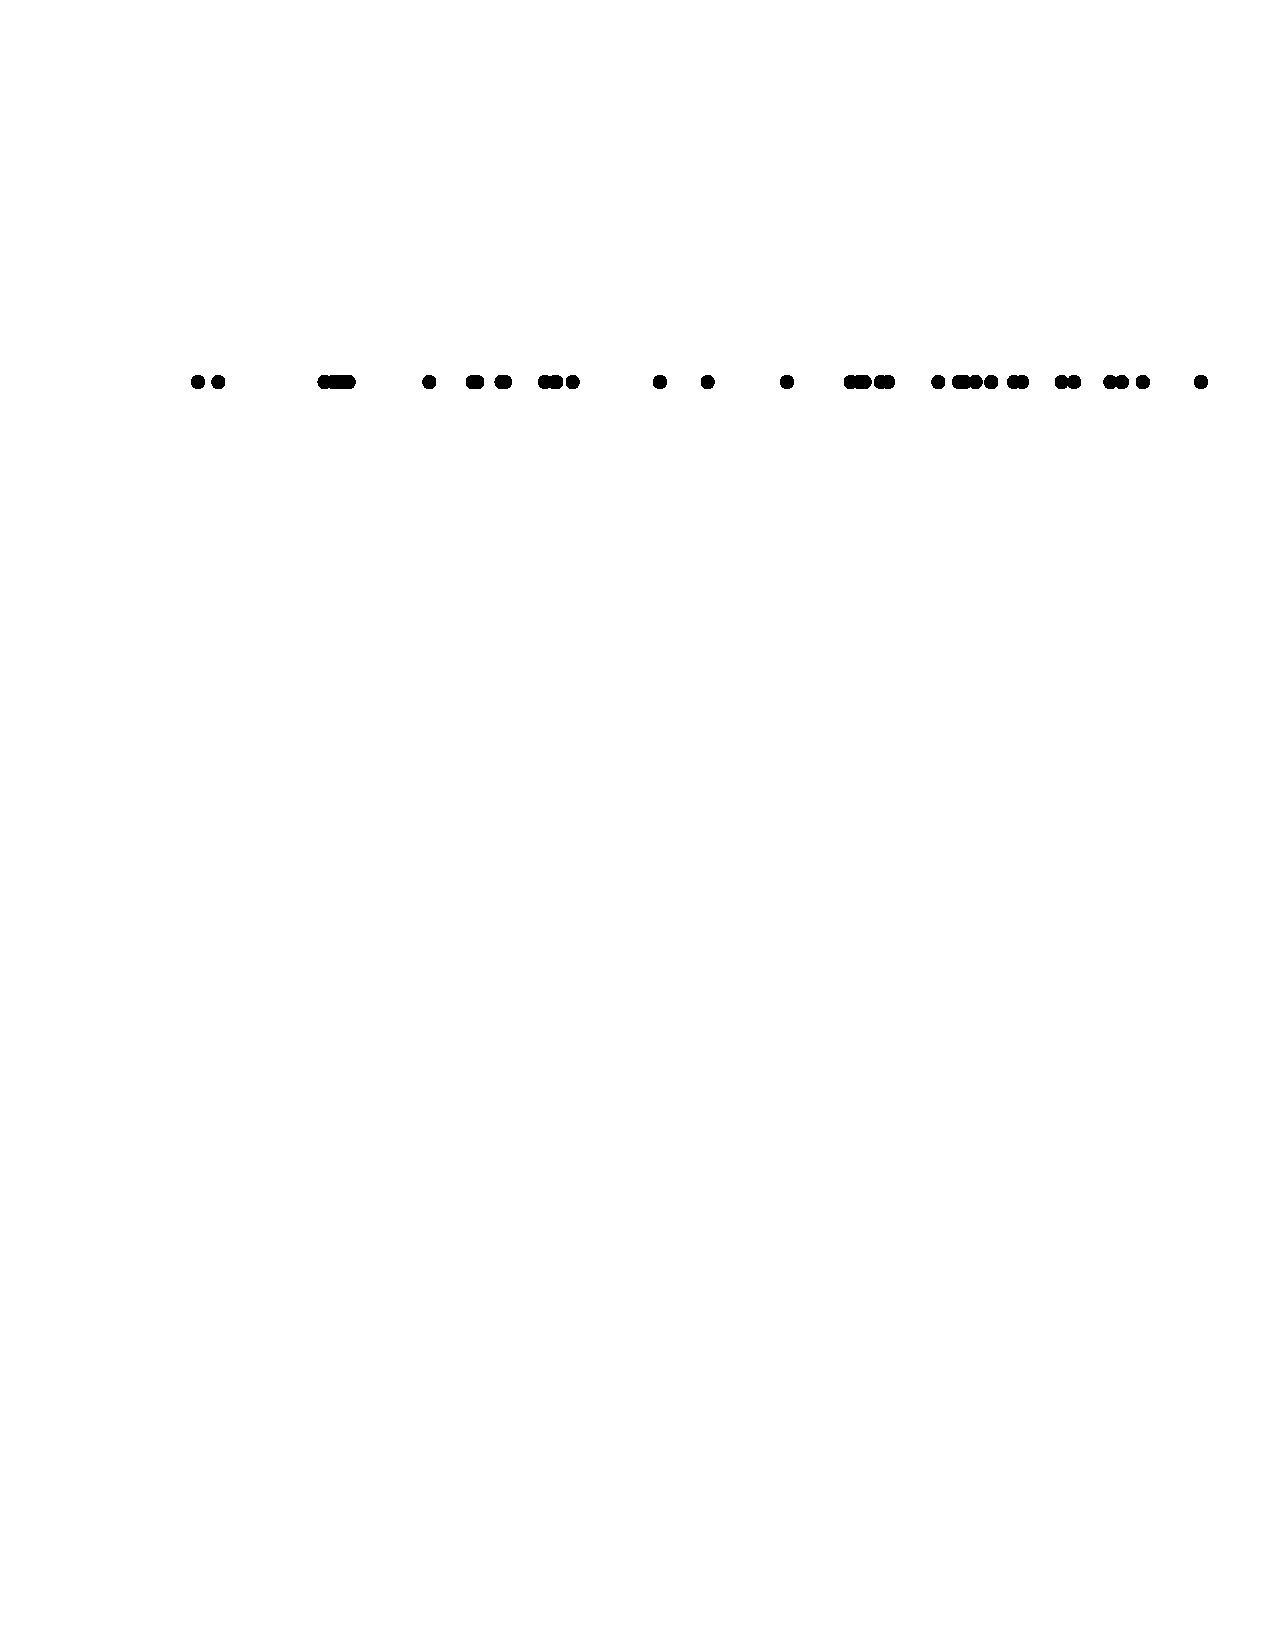
\includegraphics[width=2.5in]{images/points.pdf}
\caption{Points to cluster}
\label{fig:cluster}
\end{figure}
\begin{figure}[!h]
\centering
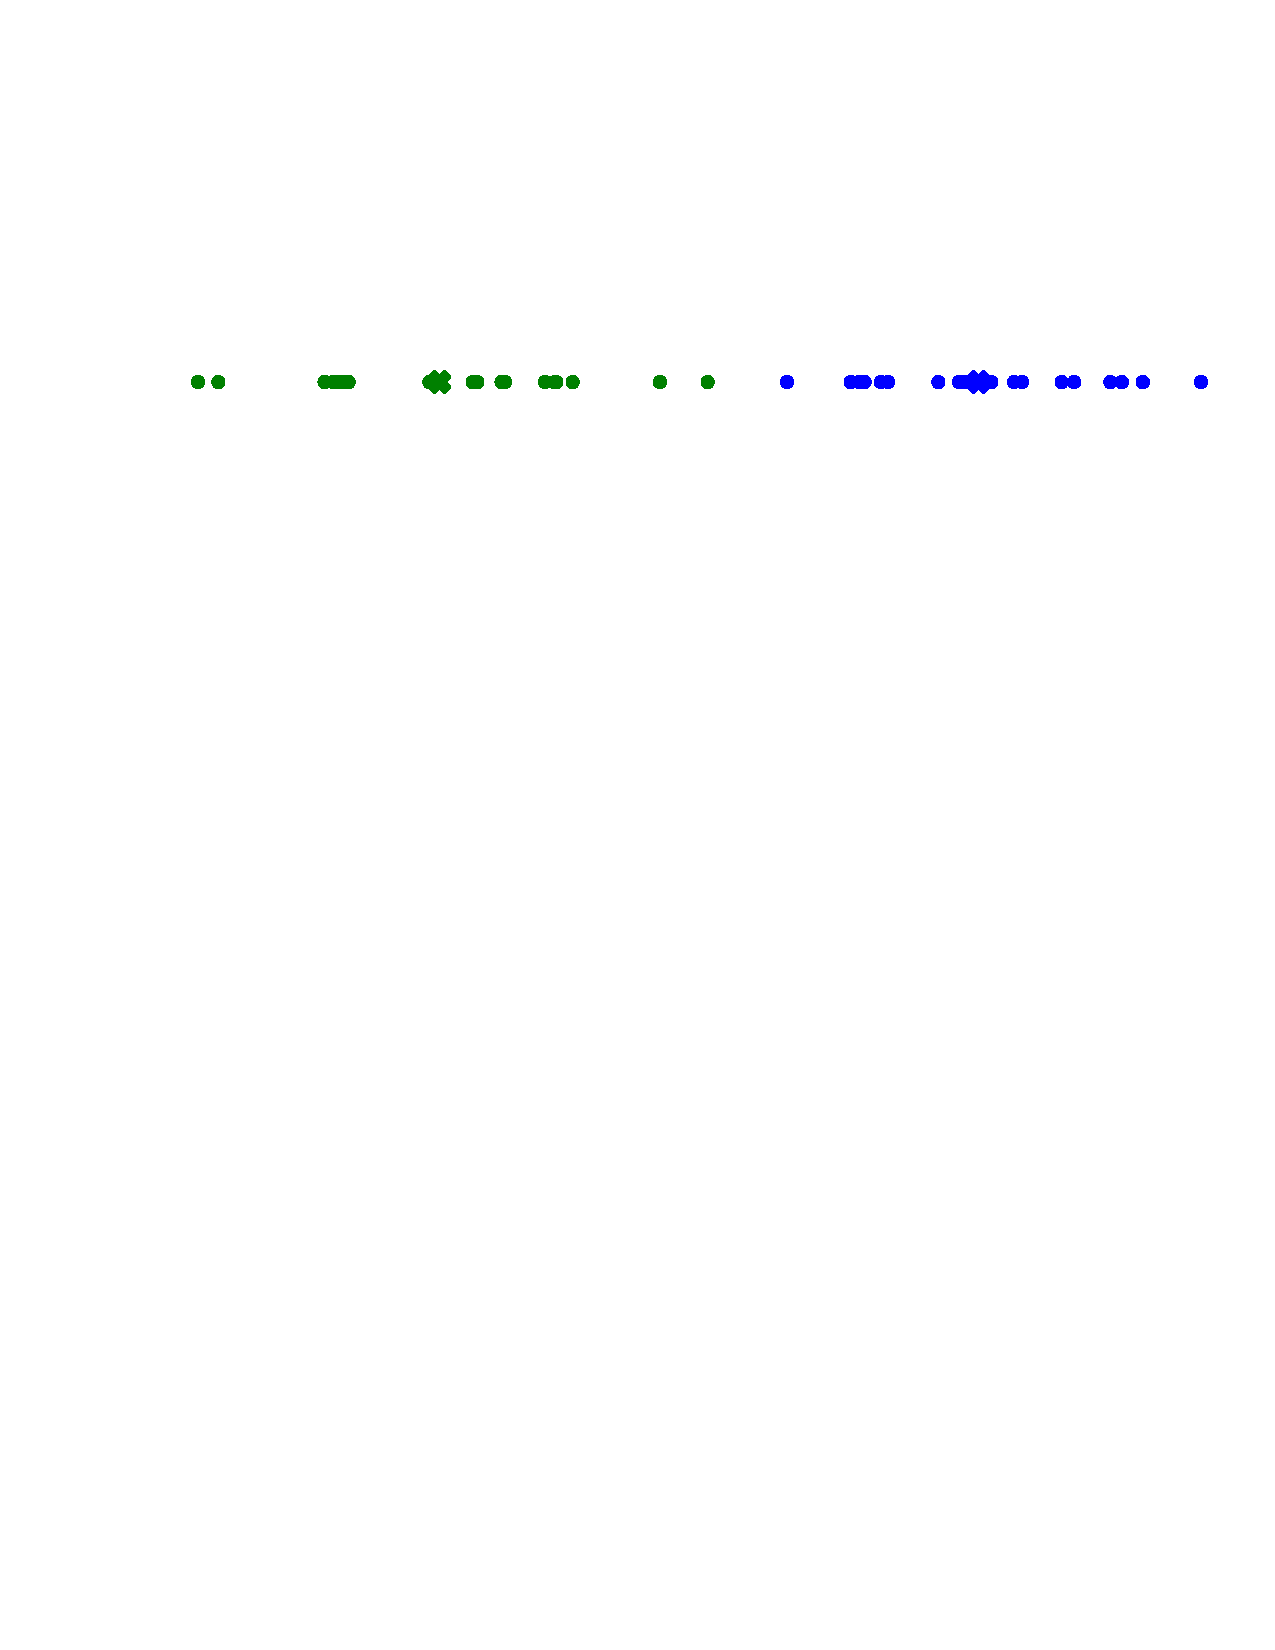
\includegraphics[width=2.5in]{images/clustered_points.pdf}
\caption{Points grouped in two clusters (green and blue). The points labelled with X represent the means of the corresponding distributions}
\label{fig:cluster}
\end{figure}

One interesting thing we found out while implementing the algorithm is that not every start state gives us this clustering. Many start states are a failure.
And I think it must be right too, because EM only finds the local optimum and not the global optimum. If our initial guess is bad then it probably will not
give the optimal value of the means. The means, variance and weights of the two Gaussians are given in the table \ref{table:parameters}.

\begin{table}[!h]
\renewcommand{\arraystretch}{0.4}
\caption{Parameters of the Gaussians}
\label{table:parameters}
\centering
\begin{tabular}{|c|c|c|c|}
\hline
{\bfseries S.No.} & {\bfseries Mean} & {\bfseries Variance} & {\bfseries Weight}\\
\hline \hline
1 & 0.7062 & 0.7155 & 0.5010\\
\hline
2 & 4.0404 & 0.4763 & 0.4989\\
\hline
\end{tabular}
\end{table}

\title{Artificial Intelligence Report on Solutions to Laboratory Problems}

\author{Siddhartha~Tiwari, Siddharth~Mani~Tiwari, Saurabh~Kumar, Pushkar~Tiwari}

%\author{
%\IEEEauthorblockN{Siddhartha Tiwari}\IEEEauthorblockA{201851127}
%\and
%\IEEEauthorblockN{Siddharth Mani Tiwari}\IEEEauthorblockA{201851126}
%\and
%\IEEEauthorblockN{Saurabh Kumar}\IEEEauthorblockA{201851113}
%\and
%\IEEEauthorblockN{Pushkar Tiwari}\IEEEauthorblockA{201851095}
%}

\section{Graph Search agent And 8 puzzle}
\subsection{To design a graph search agent and understand the use of a hash table, queue
in state space search.}

\begin{algorithm}
\caption{ Graph search algorithm}
\begin{algorithmic}
\Function{graph-search}{$search-space$}\Comment{ return solution or failure}
\State $visited \gets \{\}$
\State $frontier \gets \{start\}$ 
\While{$frontier.size$ $\neq$ 0}
\State $curr \gets frontier.dequeue()$
\If{$curr = gl$}
\State \textbf{return} $start \rightarrow curr$
\EndIf
\State $frontier.enqueue(curr.children \notin visited)$
\State $visited \gets visited + \{curr\}$
\EndWhile\label{bfsendwhile}
\EndProcedure
\end{algorithmic}
\end{algorithm}

\subsection{Flowchart}

\begin{figure}[!h]
\centering
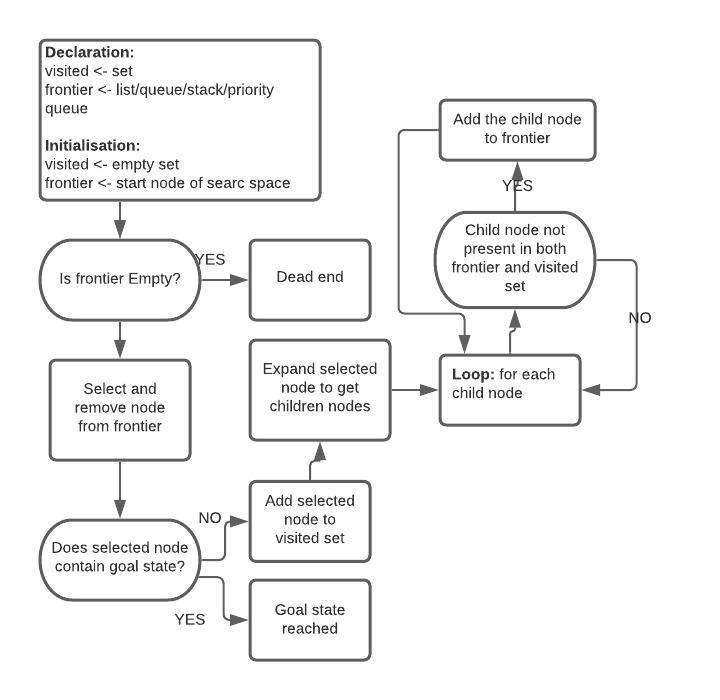
\includegraphics[width=3.5in]{images/Week1.jpeg}
\caption{Flowchart of the agent}
\label{fig_sim}
\end{figure}


\subsection{The functions imitating the environment for PUZZLE-8}
Our environment stores the goal state and then we mark the
previously visited nodes as true.

Successor states can be found using Successor() function.
\textbf{Function:} Compute heuristics\textunderscore value (state) \\
This function calculates the heuristic value of a given state.
Heuristic value is calculated as counting the number of misplaced tiles for a given state. \\

\textbf{Function:} is\textunderscore valid(x,y) \\
This function checks whether the current state transition is valid or not. \\

\textbf{Function:} successor \\
This function stores the successor of
a given node in its child by moving an empty cell in all the
possible directions. \\

\textbf{Function:} visit(State) \\
This function checks whether the state is already visited or
not.

\subsection{Iterative Deepening Search}
Iterative Deepening Search (IDS) is an iterative graph searching strategy that takes advantage of the completeness of the Breadth-First Search (BFS) strategy but uses much less memory in each iteration (similar to Depth-First Search).

IDS achieves the desired completeness by enforcing a depth-limit on DFS that mitigates the possibility of getting stuck in an infinite or a very long branch. It searches each branch of a node from left to right until it reaches the required depth. Once it has, IDS goes back to the root node and explores a different branch that is similar to DFS.\\

\begin{tabular} { | p {3 cm} | p {3 cm} | p {2 cm} | }
\hline
\multicolumn{3} { | c | }{Performance And Comparisons}\\
\hline
Uniform State Space Search Method & Time Complexity & Space Complexity \\
\hline
$BFS$ & $O(b^{d})$ & $O(b^{d})$ \\
$DFS$ & $O(b^{d})$ & $O(b.d)$ \\
Iterative Deepening Search & $O(b^{d})$ & $O(b.d)$ \\
\hline
\end{tabular}

\subsection{Considering the cost associated with every move to be the same (uniform cost), write a function which can backtrack and produce the path taken to reach the goal state from the source/ initial state.}

\textbf{Function:} Solution() \\
This function backtracks and produces the path and action
taken to reach the goal state from initial state.\\

\begin{figure}[!h]
\centering
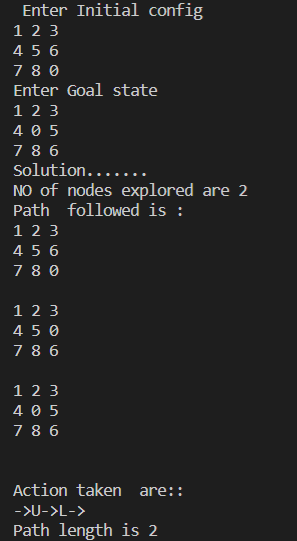
\includegraphics[width=2.5in]{images/snippet.PNG}
\caption{Path Followed}
\label{fig_sim}
\end{figure}

\subsection{Uniform Cost analysis}
Cost analysis on the basis of depth of the tree and time taken to reach the goal state and total number of nodes that are generated during this process. \\ \\

\begin{tabular} { | p {2 cm} | p {2 cm} | p {3 cm} | }
\hline
\multicolumn{3} { | c | }{Cost Analysis}\\
\hline
Depth & Time(in seconds) & Space(Nodes generated) \\
\hline
$0$ & $11.442$ & $0$\\
$1$ & $23.442$ & $3$\\
$2$ & $31.932$ & $6$\\
$3$ & $33.08$ & $9$\\
$4$ & $56.53$ & $13$\\
$5$ & $45.30$ & $15$\\
$6$ & $38.30$ & $20$\\
$7$ & $43.04$ & $29$\\
$8$ & $55.29$ & $39$\\
$9$ & $31.50$ & $73$\\
$10$ & $25.56$ & $96$\\
\hline
\end{tabular}
 \\ \\

\begin{figure}[!h]
\centering
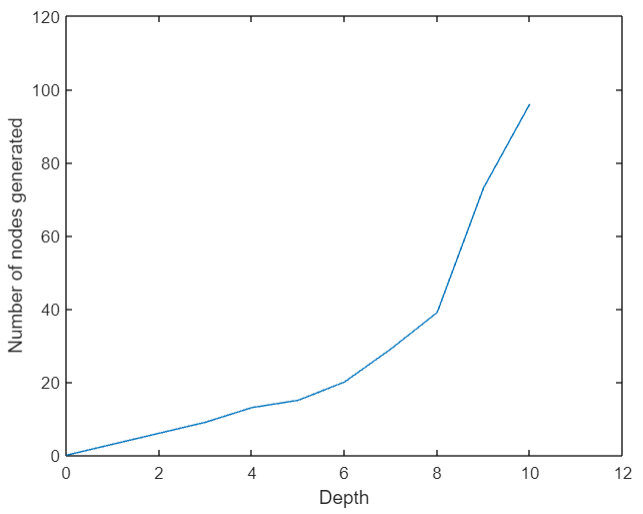
\includegraphics[width=3in]{images/graph1.PNG}
\caption{Memory requirement profile graph}
\label{fig_sim}
\end{figure}

\section{Matchbox Educable Naughts and Crosses Engine : MENACE}
\subsection{Introduction}
The Matchbox Educable Noughts and Crosses Engine or MENACE was a mechanical computer made from 304 matchboxes.It was designed to play human opponents in games of noughts and crosses (tic-tac-toe) by returning a move for any given state of play and to refine its strategy through reinforcement learning.
Each of the matchboxes contains a number of coloured
beads, each colour representing a valid move Menace could
play for corresponding board layout. The starting number of
beads in each matchbox varies depending on the number of
turns that have already been played.

\subsection{Initial Configuration}
For each configuration of the tic-tac-toe game, we have to
have a matchbox. The number of match box required can be
very large as the number of possible “game states” is a large
number ($3^{9} = 19683$). However, this number can be reduced
if we apply the fact that some game states will never appear
if the winning state comes before that and some game states
we dont have to count .Once we have the matchboxes, we will
throw away the match sticks and put some beads of 9 different
colors. Each colour should have more or less equal number of
beads inside the box . Each color will represent a unique box
on the board.In Donald Michie’s original version of Menace,
the box representing Menace’s first turn had four beads for
each different move. The boxes representing the layouts of the
board for Menace’s second turn contained three beads for each
different move; there were two beads each for Menace’s third;
and one of each in the boxes representing Menace’s fourth go.
There are no boxes representing Menace’s fifth move as there
is only one space remaining and Menace is forced to take it.

\subsection{Gameplay}
\begin{itemize}
\item each tic-tac-toe board position corresponds to a matchbox.
\item at the beginning of play, each matchbox is filled will beads of different colors.
\item there are nine bead colors: one for each board position.
\item when it is MENACE’s turn, open drawer corresponding to board configuration
 and select a bead randomly. Make the corresponding move. Leave bead on
 table and leave matchbox open.

\end{itemize}

\subsection{Reward}
\begin{itemize}
\item play an entire game to its conclusion until it ends: win/lose/draw.
\item if MENACE loses the game, remove beads from table and throw them away.
\item if MENACE draws, replace each bead back into the box it came from. Add an
 extra bead of the same color to each box.
\item if MENACE wins, replace each bead back into the box it came from. Add \textbf{THREE} extra beads of the same color to each box.
\end{itemize}

\subsection{Implementation}
\begin{itemize}
\item First generate all the possible states of the game and possible moves for each of the states. This step generates a huge number of states.

\begin{figure}[!h]
\centering
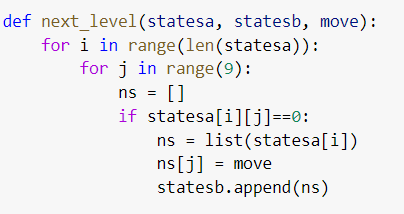
\includegraphics[width=3in]{images/states_generator.PNG}
\caption{Generate all the states}
\label{fig_sim}
\end{figure}

\item Since tic-tac-toe game board is symmetric, so many of the states are actually similar states if rotated or taken mirror image of the board. So we remove all the duplicate states that we generated. After this we are left with only around 900 states.

\item Now, the AI agent start playing games (initially with random moves and then with different strategies) with itself. 

\begin{figure}[!h]
\centering
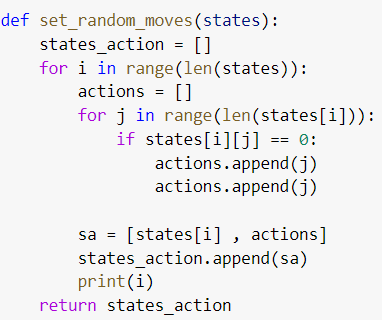
\includegraphics[width=3in]{images/Random_moves.PNG}
\caption{Playing with random moves}
\label{fig_sim}
\end{figure}

After every game, it updates all the moves corresponding to the visited states as follows:
\begin{itemize}
\item If it wins the game then it adds the corresponding move in the possible moves for that states. This increases the possibility of selecting that move again if we uniformly sample the moves for that state. Shorter the games more will be the addition of the moves. Also, closer the the step to the winning step of the game more will be the adding of the winning moves to the state.
\item If it loses the game, it deletes the corresponding moves that it has played from the states. Shorter the games more will be the deleting of the moves. Also, closer the the step to the winning step of the game more will be the deletion of the winning moves to the state.
\end{itemize}

\item Now, after thousands of self games, the states have more of the winning moves than the losing moves.
\item The system saves all the states and corresponding moves in a experience.dat file.
    
\end{itemize}
    
Before playing with human player, the system reads the experience.dat file and loads the staes and corresponding moves. Now for every state in the game, the agent plays the maximum occurring moves for that state.


\nocite{Do2008}
\nocite{HMM_Stamp}
\nocite{Menace1}
\nocite{Menace2}
\bibliography{references}
\end{document}
